\documentclass[12pt]{article}
\usepackage{graphicx,blindtext}
\usepackage[dvipsnames]{xcolor}
\usepackage[
    top=8mm,
    bottom=8mm,
    left=8mm,
    right=8mm,
    ]{geometry}
\usepackage{amssymb}
\usepackage{amsmath}
\usepackage{geometry}
\usepackage{esdiff}
\usepackage{cancel}
\usepackage{siunitx}
\usepackage{tikz}
\usetikzlibrary{calc}

\DeclareMathOperator{\di}{d\!}
\newcommand*\Eval[3]{\left.#1\right\rvert_{#2}^{#3}}
\setlength{\parindent}{0pt}

\title{Dynamics Jan 2009 Mark Scheme}
\author{Thomas Romanus}
\date{\today}

\begin{document}

    \maketitle

    Q1a.

    \begin{equation*}
        \begin{alignedat}{2}
        \underline{v_0}&=v_0(\cos\theta,\sin\theta)^T&\qquad\underline{a}&=g(0,1)^T\\
        \implies\underline{v}(t)&=(v_0cos\theta,v_0\sin\theta-gt)^T\\
        \text{At max height:  }\underline{v}(t)\cdot\hat{\underline{i}}&=0&\qquad\implies v_0\sin\theta-gt&=0\\
        \implies t&=\frac{v_0\sin\theta}{g}\qquad\text{As required.}
        \end{alignedat}
    \end{equation*}

    As parabolas are symetric then:

    \begin{equation*}
        \begin{alignedat}{1}
            T&=2t=\frac{v_0\sin\theta}{g}\\
            \underline{x}(t)&=(v_0tcos\theta,v_0t\sin\theta-\frac{gt^2}{2})^T\\
            \implies\underline{x}(T)\cdot\hat{\underline{i}}&=\frac{2v_0^2\sin\theta\cos\theta}{g}\qquad\text{As required.}
        \end{alignedat}
    \end{equation*}

    b.
    $$\underline{\tau}=\underline{r}\times\underline{F}=
    \begin{vmatrix}
        \hat{\underline{i}} & \hat{\underline{j}} & \hat{\underline{k}} \\
        7 & 3 & 1 \\
        -3 & 1 & 5
    \end{vmatrix}
    =(14,-38,16)^T\text{ Nm}
    $$

    c.

    $$\Delta KE=-\Delta GPE\implies\frac{mv_{esc.}^2}{2}=\frac{GM_{murc.}m}{R_{murc.}}\implies v_{esc.}=\sqrt{\frac{2GM_{murc.}}{R_{murc.}}}=4255\text{ ms$^{-1}$}$$

    (Note: Bottomline answer is $4254$ ms$^{-1}$ probably due to differeing $G$ values)

    di.

    No, as given a moving object the linear momentum of the system is non-zero and due to the conservation of linear momentum if one of the objects becomes stationary due to the collision then the other must be moving in order to have a non-zero final momentum.

    ii.

    Yes, if $e=1$ and masses are equal and the masses are balls and the collision is not oblique this necessitates the initially moving mass to be stationary after the collision.

    \begin{equation*}
        \begin{alignedat}{2}
            p&=v_{1i}m\text{ (i)}\qquad&\Delta v_0&=v_{1i}\text{ (ii)}\\
            \text{(i)}\implies mv_{1i}&=mv_{1f}+mv_{2f} &\implies v_{1i}&=v_{1f}+v_{2f}\qquad\text{by conservation of linear momentum}\\
            \text{(ii)}\implies -\Delta v&=-v_{1i}=v_{1f}-v_{2f}&&\text{As collision is elastic}\\
            \implies v_{1f}&=0\qquad&v_{2f}&=v_{1i}
        \end{alignedat}
    \end{equation*}

    e.

    \begin{tikzpicture}
        % Original object (e.g., a box with forces)
        \begin{scope}[shift={(0,0)}]
            \draw[thick] (0,0) rectangle (2,1) node[midway] {wagon};
            \draw[->,thick] (1,1) -- (1,2.5) node[above] {$R_w$};
            \draw[->,thick] (1,0) -- (1,-1.5) node[below] {$m_wg$};
            \draw[->,thick] (2,0.5) -- (3.5,0.5) node[right] {$T$};
            \draw[->,thick] (0,0.5) -- (-1.5,0.5) node[left] {$F_{fric}$};
        \end{scope}
        
        % Translated object (shifted by (3,2))
        \begin{scope}[shift={(7,0)}]
            \draw[thick] (0,0) rectangle (2,1) node[midway] {horse};
            \draw[->,thick] (1,1) -- (1,2.5) node[above] {$R_g$};
            \draw[->,thick] (1,0) -- (1,-1.5) node[below] {$m_hg$};
            \draw[->,thick] (2,0.5) -- (3.5,0.5) node[right] {$F_{drive}$};
            \draw[->,thick] (0,0.5) -- (-1.5,0.5) node[left] {$T$};
        \end{scope}
        
    \end{tikzpicture}

    The foreces labelled $T$ on both diagrams are N3L pairs.

    The groups with equal magnitudes are: $T$, $F_{fric}$, and $F_{drive}$; $R_w$, and $m_wg$; and $R_h$, and $m_hg$.

    2a.

    \begin{center}
        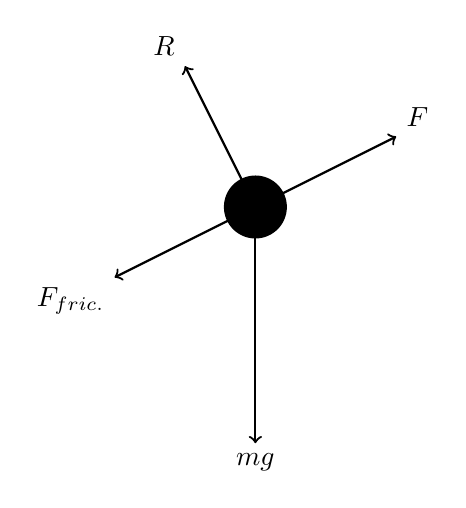
\begin{tikzpicture}[scale=2]
            \def\theta{26.565} % Define the slope angle
        
            % Draw a small black filled circle at (1.5,1)
            \fill (1.5,1) circle (0.2);
        
            % Draw the forces with labels at the ends of the arrows
            \draw[->, thick] (1.5,1) -- ++(\theta:1cm) node[above right] {$F$}; % Tension force
            \draw[->, thick] (1.5,1) -- ++(-90:1.5cm) node[below] {$mg$}; % Gravitational force
            \draw[->, thick] (1.5,1) -- ++(\theta + 90:1cm) node[above left] {$R$}; % Normal force
            \draw[->, thick] (1.5,1) -- ++(\theta + 180:1cm) node[below left] {$F_{fric.}$}; % Frictional force
        
        \end{tikzpicture}
    \end{center}

    b.

    \[F_{res.}=\alpha t^2+\beta-mg(\sin30^\circ-\mu_k\cos30^\circ)\]

    c.

    \begin{equation*}
        \begin{alignedat}{2}
            I=
        \end{alignedat}
    \end{equation*}

\end{document}